\begin{figure}[h!]
    \centering
    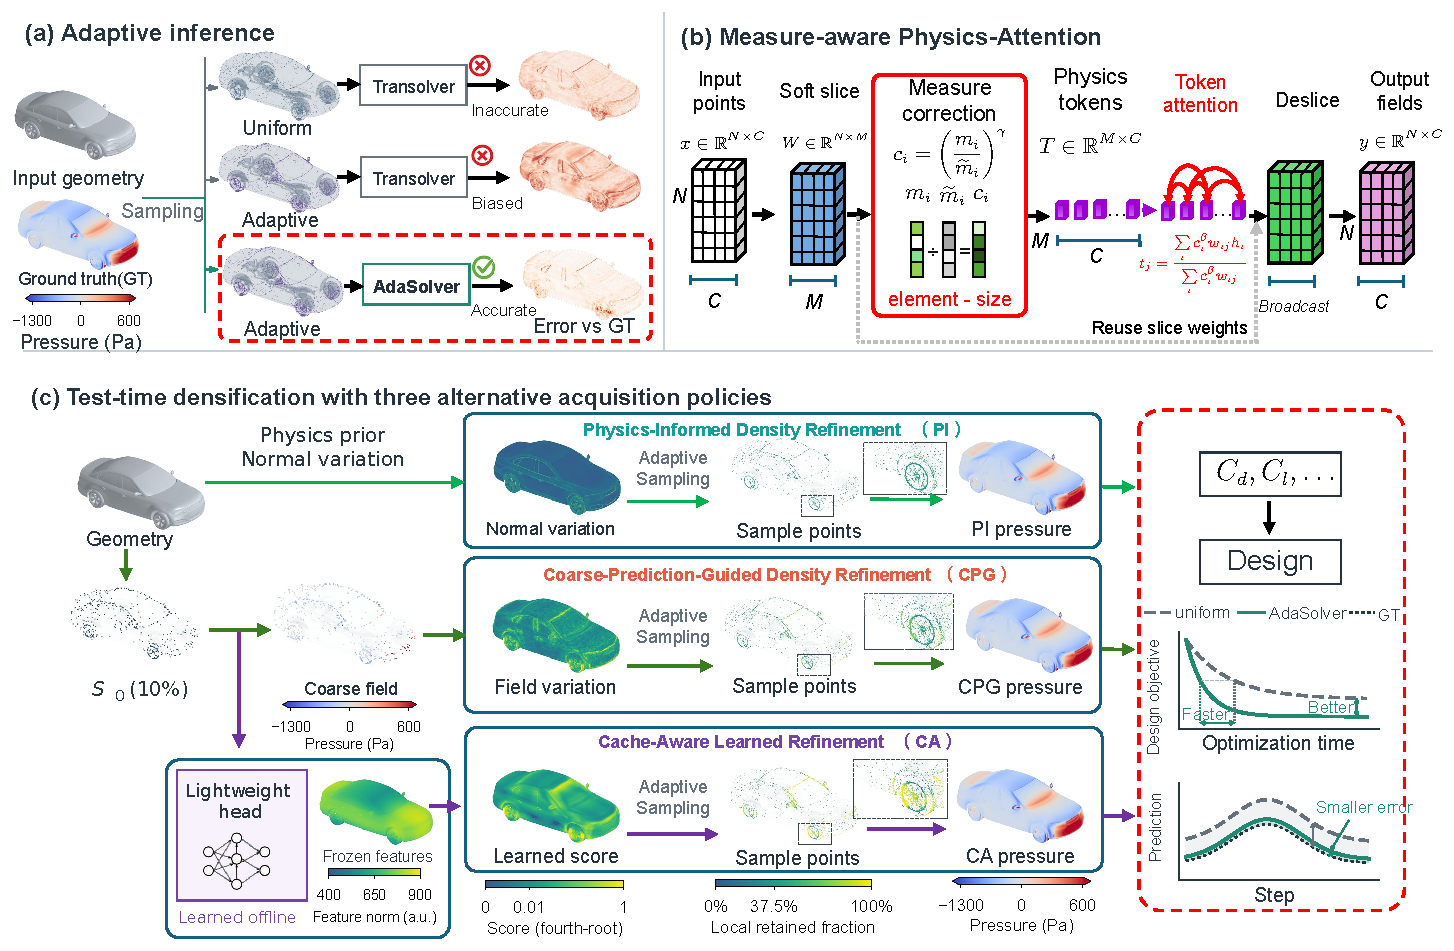
\includegraphics[width=\linewidth]{figures/fig1_overview.pdf}
    \caption{\textbf{AdaSolver overview.}
    (a) Adaptive inference with measure correction.
    (b) Corrected aggregation, token attention, and deslicing.
    (c) Geometry priors, coarse predictions, and a lightweight head on frozen
    features provide alternative refinement signals. The frozen operator evaluates
    the selected points and supplies aerodynamic quantities for design. The
    rightmost curves illustrate the design objectives schematically.}
    \label{fig:adasolver_overview}
\end{figure}
